\documentclass[1p]{elsarticle_modified}
%\bibliographystyle{elsarticle-num}

%\usepackage[colorlinks]{hyperref}
%\usepackage{abbrmath_seonhwa} %\Abb, \Ascr, \Acal ,\Abf, \Afrak
\usepackage{amsfonts}
\usepackage{amssymb}
\usepackage{amsmath}
\usepackage{amsthm}
\usepackage{scalefnt}
\usepackage{amsbsy}
\usepackage{kotex}
\usepackage{caption}
\usepackage{subfig}
\usepackage{color}
\usepackage{graphicx}
\usepackage{xcolor} %% white, black, red, green, blue, cyan, magenta, yellow
\usepackage{float}
\usepackage{setspace}
\usepackage{hyperref}

\usepackage{tikz}
\usetikzlibrary{arrows}

\usepackage{multirow}
\usepackage{array} % fixed length table
\usepackage{hhline}

%%%%%%%%%%%%%%%%%%%%%
\makeatletter
\renewcommand*\env@matrix[1][\arraystretch]{%
	\edef\arraystretch{#1}%
	\hskip -\arraycolsep
	\let\@ifnextchar\new@ifnextchar
	\array{*\c@MaxMatrixCols c}}
\makeatother %https://tex.stackexchange.com/questions/14071/how-can-i-increase-the-line-spacing-in-a-matrix
%%%%%%%%%%%%%%%

\usepackage[normalem]{ulem}

\newcommand{\msout}[1]{\ifmmode\text{\sout{\ensuremath{#1}}}\else\sout{#1}\fi}
%SOURCE: \msout is \stkout macro in https://tex.stackexchange.com/questions/20609/strikeout-in-math-mode

\newcommand{\cancel}[1]{
	\ifmmode
	{\color{red}\msout{#1}}
	\else
	{\color{red}\sout{#1}}
	\fi
}

\newcommand{\add}[1]{
	{\color{blue}\uwave{#1}}
}

\newcommand{\replace}[2]{
	\ifmmode
	{\color{red}\msout{#1}}{\color{blue}\uwave{#2}}
	\else
	{\color{red}\sout{#1}}{\color{blue}\uwave{#2}}
	\fi
}

\newcommand{\Sol}{\mathcal{S}} %segment
\newcommand{\D}{D} %diagram
\newcommand{\A}{\mathcal{A}} %arc


%%%%%%%%%%%%%%%%%%%%%%%%%%%%%5 test

\def\sl{\operatorname{\textup{SL}}(2,\Cbb)}
\def\psl{\operatorname{\textup{PSL}}(2,\Cbb)}
\def\quan{\mkern 1mu \triangleright \mkern 1mu}

\theoremstyle{definition}
\newtheorem{thm}{Theorem}[section]
\newtheorem{prop}[thm]{Proposition}
\newtheorem{lem}[thm]{Lemma}
\newtheorem{ques}[thm]{Question}
\newtheorem{cor}[thm]{Corollary}
\newtheorem{defn}[thm]{Definition}
\newtheorem{exam}[thm]{Example}
\newtheorem{rmk}[thm]{Remark}
\newtheorem{alg}[thm]{Algorithm}

\newcommand{\I}{\sqrt{-1}}
\begin{document}

%\begin{frontmatter}
%
%\title{Boundary parabolic representations of knots up to 8 crossings}
%
%%% Group authors per affiliation:
%\author{Yunhi Cho} 
%\address{Department of Mathematics, University of Seoul, Seoul, Korea}
%\ead{yhcho@uos.ac.kr}
%
%
%\author{Seonhwa Kim} %\fnref{s_kim}}
%\address{Center for Geometry and Physics, Institute for Basic Science, Pohang, 37673, Korea}
%\ead{ryeona17@ibs.re.kr}
%
%\author{Hyuk Kim}
%\address{Department of Mathematical Sciences, Seoul National University, Seoul 08826, Korea}
%\ead{hyukkim@snu.ac.kr}
%
%\author{Seokbeom Yoon}
%\address{Department of Mathematical Sciences, Seoul National University, Seoul, 08826,  Korea}
%\ead{sbyoon15@snu.ac.kr}
%
%\begin{abstract}
%We find all boundary parabolic representation of knots up to 8 crossings.
%
%\end{abstract}
%\begin{keyword}
%    \MSC[2010] 57M25 
%\end{keyword}
%
%\end{frontmatter}

%\linenumbers
%\tableofcontents
%
\newcommand\colored[1]{\textcolor{white}{\rule[-0.35ex]{0.8em}{1.4ex}}\kern-0.8em\color{red} #1}%
%\newcommand\colored[1]{\textcolor{white}{ #1}\kern-2.17ex	\textcolor{white}{ #1}\kern-1.81ex	\textcolor{white}{ #1}\kern-2.15ex\color{red}#1	}

{\Large $\underline{12a_{0777}~(K12a_{0777})}$}

\setlength{\tabcolsep}{10pt}
\renewcommand{\arraystretch}{1.6}
\vspace{1cm}\begin{tabular}{m{100pt}>{\centering\arraybackslash}m{274pt}}
\multirow{5}{120pt}{
	\centering
	\includegraphics[width=112pt]{../../../GIT/diagram.site/Diagrams/png/1578_12a_0777.png}\\
\ \ \ A knot diagram\footnotemark}&
\allowdisplaybreaks
\textbf{Linearized knot diagam} \\
\cline{2-2}
 &
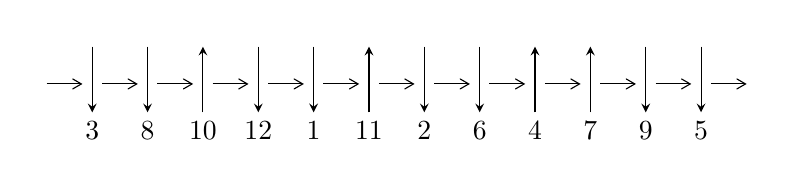
\begin{tikzpicture}[x=20pt, y=17pt]
	% nodes
	\node (C0) at (0, 0) {};
	\node (C1) at (1, 0) {};
	\node (C1U) at (1, +1) {};
	\node (C1D) at (1, -1) {3};

	\node (C2) at (2, 0) {};
	\node (C2U) at (2, +1) {};
	\node (C2D) at (2, -1) {8};

	\node (C3) at (3, 0) {};
	\node (C3U) at (3, +1) {};
	\node (C3D) at (3, -1) {10};

	\node (C4) at (4, 0) {};
	\node (C4U) at (4, +1) {};
	\node (C4D) at (4, -1) {12};

	\node (C5) at (5, 0) {};
	\node (C5U) at (5, +1) {};
	\node (C5D) at (5, -1) {1};

	\node (C6) at (6, 0) {};
	\node (C6U) at (6, +1) {};
	\node (C6D) at (6, -1) {11};

	\node (C7) at (7, 0) {};
	\node (C7U) at (7, +1) {};
	\node (C7D) at (7, -1) {2};

	\node (C8) at (8, 0) {};
	\node (C8U) at (8, +1) {};
	\node (C8D) at (8, -1) {6};

	\node (C9) at (9, 0) {};
	\node (C9U) at (9, +1) {};
	\node (C9D) at (9, -1) {4};

	\node (C10) at (10, 0) {};
	\node (C10U) at (10, +1) {};
	\node (C10D) at (10, -1) {7};

	\node (C11) at (11, 0) {};
	\node (C11U) at (11, +1) {};
	\node (C11D) at (11, -1) {9};

	\node (C12) at (12, 0) {};
	\node (C12U) at (12, +1) {};
	\node (C12D) at (12, -1) {5};
	\node (C13) at (13, 0) {};

	% arrows
	\draw[->,>={angle 60}]
	(C0) edge (C1) (C1) edge (C2) (C2) edge (C3) (C3) edge (C4) (C4) edge (C5) (C5) edge (C6) (C6) edge (C7) (C7) edge (C8) (C8) edge (C9) (C9) edge (C10) (C10) edge (C11) (C11) edge (C12) (C12) edge (C13) ;	\draw[->,>=stealth]
	(C1U) edge (C1D) (C2U) edge (C2D) (C3D) edge (C3U) (C4U) edge (C4D) (C5U) edge (C5D) (C6D) edge (C6U) (C7U) edge (C7D) (C8U) edge (C8D) (C9D) edge (C9U) (C10D) edge (C10U) (C11U) edge (C11D) (C12U) edge (C12D) ;
	\end{tikzpicture} \\
\hhline{~~} \\& 
\textbf{Solving Sequence} \\ \cline{2-2} 
 &
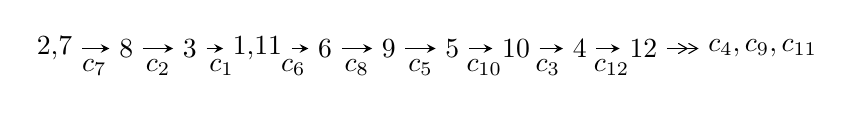
\begin{tikzpicture}[x=23pt, y=7pt]
	% node
	\node (A0) at (-1/8, 0) {2,7};
	\node (A1) at (1, 0) {8};
	\node (A2) at (2, 0) {3};
	\node (A3) at (49/16, 0) {1,11};
	\node (A4) at (33/8, 0) {6};
	\node (A5) at (41/8, 0) {9};
	\node (A6) at (49/8, 0) {5};
	\node (A7) at (57/8, 0) {10};
	\node (A8) at (65/8, 0) {4};
	\node (A9) at (73/8, 0) {12};
	\node (C1) at (1/2, -1) {$c_{7}$};
	\node (C2) at (3/2, -1) {$c_{2}$};
	\node (C3) at (5/2, -1) {$c_{1}$};
	\node (C4) at (29/8, -1) {$c_{6}$};
	\node (C5) at (37/8, -1) {$c_{8}$};
	\node (C6) at (45/8, -1) {$c_{5}$};
	\node (C7) at (53/8, -1) {$c_{10}$};
	\node (C8) at (61/8, -1) {$c_{3}$};
	\node (C9) at (69/8, -1) {$c_{12}$};
	\node (A10) at (11, 0) {$c_{4},c_{9},c_{11}$};

	% edge
	\draw[->,>=stealth]	
	(A0) edge (A1) (A1) edge (A2) (A2) edge (A3) (A3) edge (A4) (A4) edge (A5) (A5) edge (A6) (A6) edge (A7) (A7) edge (A8) (A8) edge (A9) ;
	\draw[->>,>={angle 60}]	
	(A9) edge (A10);
\end{tikzpicture} \\ 

\end{tabular} \\

\footnotetext{
The image of knot diagram is generated by the software ``\textbf{Draw programme}" developed by Andrew Bartholomew(\url{http://www.layer8.co.uk/maths/draw/index.htm\#Running-draw}), where we modified some parts for our purpose(\url{https://github.com/CATsTAILs/LinksPainter}).
}\phantom \\ \newline 
\centering \textbf{Ideals for irreducible components\footnotemark of $X_{\text{par}}$} 
 
\begin{align*}
I^u_{1}&=\langle 
8.31484\times10^{237} u^{117}-3.93039\times10^{237} u^{116}+\cdots+1.72854\times10^{239} b+2.06492\times10^{240},\\
\phantom{I^u_{1}}&\phantom{= \langle  }6.89267\times10^{239} u^{117}-1.82120\times10^{240} u^{116}+\cdots+1.01984\times10^{241} a+1.75868\times10^{242},\\
\phantom{I^u_{1}}&\phantom{= \langle  }u^{118}- u^{117}+\cdots+167 u-59\rangle \\
I^u_{2}&=\langle 
106243 u^{29}+47719 u^{28}+\cdots+20891 b-107527,\\
\phantom{I^u_{2}}&\phantom{= \langle  }-48402 u^{29}-89702 u^{28}+\cdots+20891 a+137421,\;u^{30}-8 u^{28}+\cdots+u+1\rangle \\
\\
\end{align*}
\raggedright * 2 irreducible components of $\dim_{\mathbb{C}}=0$, with total 148 representations.\\
\footnotetext{All coefficients of polynomials are rational numbers. But the coefficients are sometimes approximated in decimal forms when there is not enough margin.}
\newpage
\renewcommand{\arraystretch}{1}
\centering \section*{I. $I^u_{1}= \langle 8.31\times10^{237} u^{117}-3.93\times10^{237} u^{116}+\cdots+1.73\times10^{239} b+2.06\times10^{240},\;6.89\times10^{239} u^{117}-1.82\times10^{240} u^{116}+\cdots+1.02\times10^{241} a+1.76\times10^{242},\;u^{118}- u^{117}+\cdots+167 u-59 \rangle$}
\flushleft \textbf{(i) Arc colorings}\\
\begin{tabular}{m{7pt} m{180pt} m{7pt} m{180pt} }
\flushright $a_{2}=$&$\begin{pmatrix}0\\u\end{pmatrix}$ \\
\flushright $a_{7}=$&$\begin{pmatrix}1\\0\end{pmatrix}$ \\
\flushright $a_{8}=$&$\begin{pmatrix}1\\u^2\end{pmatrix}$ \\
\flushright $a_{3}=$&$\begin{pmatrix}- u\\- u^3+u\end{pmatrix}$ \\
\flushright $a_{1}=$&$\begin{pmatrix}u^3\\u^5- u^3+u\end{pmatrix}$ \\
\flushright $a_{11}=$&$\begin{pmatrix}-0.0675860 u^{117}+0.178577 u^{116}+\cdots-2.71344 u-17.2448\\-0.0481033 u^{117}+0.0227382 u^{116}+\cdots+4.60746 u-11.9460\end{pmatrix}$ \\
\flushright $a_{6}=$&$\begin{pmatrix}1.35041 u^{117}-0.254370 u^{116}+\cdots-160.672 u+105.956\\0.468192 u^{117}-0.0130686 u^{116}+\cdots-88.1432 u+45.9964\end{pmatrix}$ \\
\flushright $a_{9}=$&$\begin{pmatrix}-0.301176 u^{117}+0.0594844 u^{116}+\cdots+29.6650 u-1.93634\\0.133068 u^{117}-0.0786827 u^{116}+\cdots-11.8488 u+17.9718\end{pmatrix}$ \\
\flushright $a_{5}=$&$\begin{pmatrix}1.18359 u^{117}-0.271232 u^{116}+\cdots-124.787 u+85.1168\\0.193309 u^{117}+0.0423118 u^{116}+\cdots-47.5214 u+20.4555\end{pmatrix}$ \\
\flushright $a_{10}=$&$\begin{pmatrix}-0.0194826 u^{117}+0.155839 u^{116}+\cdots-7.32090 u-5.29873\\-0.0481033 u^{117}+0.0227382 u^{116}+\cdots+4.60746 u-11.9460\end{pmatrix}$ \\
\flushright $a_{4}=$&$\begin{pmatrix}0.991454 u^{117}-0.0984787 u^{116}+\cdots-165.840 u+97.9375\\0.654324 u^{117}-0.180806 u^{116}+\cdots-78.3906 u+51.7689\end{pmatrix}$ \\
\flushright $a_{12}=$&$\begin{pmatrix}-1.16560 u^{117}+0.469100 u^{116}+\cdots+122.223 u-87.0159\\-0.559715 u^{117}+0.139939 u^{116}+\cdots+69.8418 u-42.6384\end{pmatrix}$\\&\end{tabular}
\flushleft \textbf{(ii) Obstruction class $= -1$}\\~\\
\flushleft \textbf{(iii) Cusp Shapes $= 0.159031 u^{117}+0.176866 u^{116}+\cdots-8.92642 u-11.8415$}\\~\\
\newpage\renewcommand{\arraystretch}{1}
\flushleft \textbf{(iv) u-Polynomials at the component}\newline \\
\begin{tabular}{m{50pt}|m{274pt}}
Crossings & \hspace{64pt}u-Polynomials at each crossing \\
\hline $$\begin{aligned}c_{1}\end{aligned}$$&$\begin{aligned}
&u^{118}+59 u^{117}+\cdots+64351 u+3481
\end{aligned}$\\
\hline $$\begin{aligned}c_{2},c_{7}\end{aligned}$$&$\begin{aligned}
&u^{118}+u^{117}+\cdots-167 u-59
\end{aligned}$\\
\hline $$\begin{aligned}c_{3},c_{9}\end{aligned}$$&$\begin{aligned}
&u^{118}+u^{117}+\cdots-681405 u-118739
\end{aligned}$\\
\hline $$\begin{aligned}c_{4},c_{5},c_{12}\end{aligned}$$&$\begin{aligned}
&u^{118}+3 u^{117}+\cdots+30 u-1
\end{aligned}$\\
\hline $$\begin{aligned}c_{6},c_{10}\end{aligned}$$&$\begin{aligned}
&u^{118}-2 u^{117}+\cdots+46028 u+3241
\end{aligned}$\\
\hline $$\begin{aligned}c_{8}\end{aligned}$$&$\begin{aligned}
&u^{118}-9 u^{117}+\cdots-6352773 u+341129
\end{aligned}$\\
\hline $$\begin{aligned}c_{11}\end{aligned}$$&$\begin{aligned}
&u^{118}-6 u^{117}+\cdots-1478146065 u+117887275
\end{aligned}$\\
\hline
\end{tabular}\\~\\
\newpage\renewcommand{\arraystretch}{1}
\flushleft \textbf{(v) Riley Polynomials at the component}\newline \\
\begin{tabular}{m{50pt}|m{274pt}}
Crossings & \hspace{64pt}Riley Polynomials at each crossing \\
\hline $$\begin{aligned}c_{1}\end{aligned}$$&$\begin{aligned}
&y^{118}+13 y^{117}+\cdots+257101793 y+12117361
\end{aligned}$\\
\hline $$\begin{aligned}c_{2},c_{7}\end{aligned}$$&$\begin{aligned}
&y^{118}-59 y^{117}+\cdots-64351 y+3481
\end{aligned}$\\
\hline $$\begin{aligned}c_{3},c_{9}\end{aligned}$$&$\begin{aligned}
&y^{118}+105 y^{117}+\cdots+500751984721 y+14098950121
\end{aligned}$\\
\hline $$\begin{aligned}c_{4},c_{5},c_{12}\end{aligned}$$&$\begin{aligned}
&y^{118}-125 y^{117}+\cdots-110 y+1
\end{aligned}$\\
\hline $$\begin{aligned}c_{6},c_{10}\end{aligned}$$&$\begin{aligned}
&y^{118}+80 y^{117}+\cdots+87494132 y+10504081
\end{aligned}$\\
\hline $$\begin{aligned}c_{8}\end{aligned}$$&$\begin{aligned}
&y^{118}-35 y^{117}+\cdots-4220593276107 y+116368994641
\end{aligned}$\\
\hline $$\begin{aligned}c_{11}\end{aligned}$$&$\begin{aligned}
&y^{118}-60 y^{117}+\cdots-655020952466922525 y+13897409606925625
\end{aligned}$\\
\hline
\end{tabular}\\~\\
\newpage\flushleft \textbf{(vi) Complex Volumes and Cusp Shapes}
$$\begin{array}{c|c|c}  
\text{Solutions to }I^u_{1}& \I (\text{vol} + \sqrt{-1}CS) & \text{Cusp shape}\\
 \hline 
\begin{aligned}
u &= -0.178023 + 0.973643 I \\
a &= \phantom{-}0.323995 - 0.685624 I \\
b &= -0.563611 - 0.705908 I\end{aligned}
 & -4.73958 + 2.23006 I & \phantom{-0.000000 } 0 \\ \hline\begin{aligned}
u &= -0.178023 - 0.973643 I \\
a &= \phantom{-}0.323995 + 0.685624 I \\
b &= -0.563611 + 0.705908 I\end{aligned}
 & -4.73958 - 2.23006 I & \phantom{-0.000000 } 0 \\ \hline\begin{aligned}
u &= \phantom{-}0.858025 + 0.485772 I \\
a &= \phantom{-}0.645004 + 0.736781 I \\
b &= -0.906752 + 0.645911 I\end{aligned}
 & -0.61747 - 4.47528 I & \phantom{-0.000000 } 0 \\ \hline\begin{aligned}
u &= \phantom{-}0.858025 - 0.485772 I \\
a &= \phantom{-}0.645004 - 0.736781 I \\
b &= -0.906752 - 0.645911 I\end{aligned}
 & -0.61747 + 4.47528 I & \phantom{-0.000000 } 0 \\ \hline\begin{aligned}
u &= -0.977446 + 0.274662 I \\
a &= -0.05383 - 2.67293 I \\
b &= \phantom{-}0.06116 - 1.44574 I\end{aligned}
 & -7.87809 + 0.99703 I & \phantom{-0.000000 } 0 \\ \hline\begin{aligned}
u &= -0.977446 - 0.274662 I \\
a &= -0.05383 + 2.67293 I \\
b &= \phantom{-}0.06116 + 1.44574 I\end{aligned}
 & -7.87809 - 0.99703 I & \phantom{-0.000000 } 0 \\ \hline\begin{aligned}
u &= -0.334365 + 0.923343 I \\
a &= -0.213558 - 0.256070 I \\
b &= \phantom{-}0.52407 - 1.32106 I\end{aligned}
 & -4.34744 - 7.95136 I & \phantom{-0.000000 } 0 \\ \hline\begin{aligned}
u &= -0.334365 - 0.923343 I \\
a &= -0.213558 + 0.256070 I \\
b &= \phantom{-}0.52407 + 1.32106 I\end{aligned}
 & -4.34744 + 7.95136 I & \phantom{-0.000000 } 0 \\ \hline\begin{aligned}
u &= -0.962975 + 0.338096 I \\
a &= -0.893396 - 0.162256 I \\
b &= \phantom{-}0.293659 - 0.422056 I\end{aligned}
 & -3.27326 + 3.33430 I & \phantom{-0.000000 } 0 \\ \hline\begin{aligned}
u &= -0.962975 - 0.338096 I \\
a &= -0.893396 + 0.162256 I \\
b &= \phantom{-}0.293659 + 0.422056 I\end{aligned}
 & -3.27326 - 3.33430 I & \phantom{-0.000000 } 0\\
 \hline 
 \end{array}$$\newpage$$\begin{array}{c|c|c}  
\text{Solutions to }I^u_{1}& \I (\text{vol} + \sqrt{-1}CS) & \text{Cusp shape}\\
 \hline 
\begin{aligned}
u &= \phantom{-}1.020340 + 0.225366 I \\
a &= -1.70751 - 0.45340 I \\
b &= \phantom{-}0.119139 + 0.496067 I\end{aligned}
 & -10.75740 - 4.49700 I & \phantom{-0.000000 } 0 \\ \hline\begin{aligned}
u &= \phantom{-}1.020340 - 0.225366 I \\
a &= -1.70751 + 0.45340 I \\
b &= \phantom{-}0.119139 - 0.496067 I\end{aligned}
 & -10.75740 + 4.49700 I & \phantom{-0.000000 } 0 \\ \hline\begin{aligned}
u &= \phantom{-}0.195857 + 1.026490 I \\
a &= \phantom{-}0.300728 - 0.521516 I \\
b &= -0.000667 - 0.926385 I\end{aligned}
 & -3.20690 - 0.20894 I & \phantom{-0.000000 } 0 \\ \hline\begin{aligned}
u &= \phantom{-}0.195857 - 1.026490 I \\
a &= \phantom{-}0.300728 + 0.521516 I \\
b &= -0.000667 + 0.926385 I\end{aligned}
 & -3.20690 + 0.20894 I & \phantom{-0.000000 } 0 \\ \hline\begin{aligned}
u &= \phantom{-}0.285625 + 1.007520 I \\
a &= -0.269949 + 0.465828 I \\
b &= \phantom{-}0.53299 + 1.32359 I\end{aligned}
 & -11.2076 + 11.9652 I & \phantom{-0.000000 } 0 \\ \hline\begin{aligned}
u &= \phantom{-}0.285625 - 1.007520 I \\
a &= -0.269949 - 0.465828 I \\
b &= \phantom{-}0.53299 - 1.32359 I\end{aligned}
 & -11.2076 - 11.9652 I & \phantom{-0.000000 } 0 \\ \hline\begin{aligned}
u &= \phantom{-}0.516576 + 0.788684 I \\
a &= \phantom{-}0.221479 + 0.107724 I \\
b &= \phantom{-}0.032787 - 1.051840 I\end{aligned}
 & -3.49244 + 0.29145 I & \phantom{-0.000000 } 0 \\ \hline\begin{aligned}
u &= \phantom{-}0.516576 - 0.788684 I \\
a &= \phantom{-}0.221479 - 0.107724 I \\
b &= \phantom{-}0.032787 + 1.051840 I\end{aligned}
 & -3.49244 - 0.29145 I & \phantom{-0.000000 } 0 \\ \hline\begin{aligned}
u &= \phantom{-}1.033500 + 0.229710 I \\
a &= \phantom{-}1.17745 + 3.29186 I \\
b &= \phantom{-}0.127765 + 1.060230 I\end{aligned}
 & -10.73850 + 3.13540 I & \phantom{-0.000000 } 0 \\ \hline\begin{aligned}
u &= \phantom{-}1.033500 - 0.229710 I \\
a &= \phantom{-}1.17745 - 3.29186 I \\
b &= \phantom{-}0.127765 - 1.060230 I\end{aligned}
 & -10.73850 - 3.13540 I & \phantom{-0.000000 } 0\\
 \hline 
 \end{array}$$\newpage$$\begin{array}{c|c|c}  
\text{Solutions to }I^u_{1}& \I (\text{vol} + \sqrt{-1}CS) & \text{Cusp shape}\\
 \hline 
\begin{aligned}
u &= -0.683401 + 0.822336 I \\
a &= \phantom{-}0.629727 - 1.005500 I \\
b &= -0.437187 - 0.953141 I\end{aligned}
 & -4.86789 + 2.12575 I & \phantom{-0.000000 } 0 \\ \hline\begin{aligned}
u &= -0.683401 - 0.822336 I \\
a &= \phantom{-}0.629727 + 1.005500 I \\
b &= -0.437187 + 0.953141 I\end{aligned}
 & -4.86789 - 2.12575 I & \phantom{-0.000000 } 0 \\ \hline\begin{aligned}
u &= -1.017520 + 0.341721 I \\
a &= \phantom{-}1.34641 - 2.28434 I \\
b &= \phantom{-}0.037618 - 1.069500 I\end{aligned}
 & -3.51249 - 1.10895 I & \phantom{-0.000000 } 0 \\ \hline\begin{aligned}
u &= -1.017520 - 0.341721 I \\
a &= \phantom{-}1.34641 + 2.28434 I \\
b &= \phantom{-}0.037618 + 1.069500 I\end{aligned}
 & -3.51249 + 1.10895 I & \phantom{-0.000000 } 0 \\ \hline\begin{aligned}
u &= \phantom{-}0.516963 + 0.762482 I \\
a &= \phantom{-}0.365457 + 0.019237 I \\
b &= -0.632025 - 0.008821 I\end{aligned}
 & -2.46513 + 1.44951 I & \phantom{-0.000000 } 0 \\ \hline\begin{aligned}
u &= \phantom{-}0.516963 - 0.762482 I \\
a &= \phantom{-}0.365457 - 0.019237 I \\
b &= -0.632025 + 0.008821 I\end{aligned}
 & -2.46513 - 1.44951 I & \phantom{-0.000000 } 0 \\ \hline\begin{aligned}
u &= \phantom{-}0.772499 + 0.483784 I \\
a &= \phantom{-}0.612327 - 0.823187 I \\
b &= \phantom{-}0.769941 + 0.423078 I\end{aligned}
 & -0.346230 + 0.449095 I & \phantom{-0.000000 } 0 \\ \hline\begin{aligned}
u &= \phantom{-}0.772499 - 0.483784 I \\
a &= \phantom{-}0.612327 + 0.823187 I \\
b &= \phantom{-}0.769941 - 0.423078 I\end{aligned}
 & -0.346230 - 0.449095 I & \phantom{-0.000000 } 0 \\ \hline\begin{aligned}
u &= -0.921937 + 0.582429 I \\
a &= \phantom{-}0.168922 + 0.707460 I \\
b &= \phantom{-}0.706492 - 0.108001 I\end{aligned}
 & \phantom{-}1.55846 + 3.67318 I & \phantom{-0.000000 } 0 \\ \hline\begin{aligned}
u &= -0.921937 - 0.582429 I \\
a &= \phantom{-}0.168922 - 0.707460 I \\
b &= \phantom{-}0.706492 + 0.108001 I\end{aligned}
 & \phantom{-}1.55846 - 3.67318 I & \phantom{-0.000000 } 0\\
 \hline 
 \end{array}$$\newpage$$\begin{array}{c|c|c}  
\text{Solutions to }I^u_{1}& \I (\text{vol} + \sqrt{-1}CS) & \text{Cusp shape}\\
 \hline 
\begin{aligned}
u &= -0.682462 + 0.590348 I \\
a &= \phantom{-}0.500722 - 0.345322 I \\
b &= -0.687773 - 0.324268 I\end{aligned}
 & \phantom{-}2.26273 + 0.98072 I & \phantom{-0.000000 } 0 \\ \hline\begin{aligned}
u &= -0.682462 - 0.590348 I \\
a &= \phantom{-}0.500722 + 0.345322 I \\
b &= -0.687773 + 0.324268 I\end{aligned}
 & \phantom{-}2.26273 - 0.98072 I & \phantom{-0.000000 } 0 \\ \hline\begin{aligned}
u &= -0.783078 + 0.781095 I \\
a &= \phantom{-}0.182632 - 0.707430 I \\
b &= \phantom{-}0.477682 - 0.623977 I\end{aligned}
 & -5.18250 + 3.74930 I & \phantom{-0.000000 } 0 \\ \hline\begin{aligned}
u &= -0.783078 - 0.781095 I \\
a &= \phantom{-}0.182632 + 0.707430 I \\
b &= \phantom{-}0.477682 + 0.623977 I\end{aligned}
 & -5.18250 - 3.74930 I & \phantom{-0.000000 } 0 \\ \hline\begin{aligned}
u &= \phantom{-}1.105550 + 0.136685 I \\
a &= -0.75559 - 2.55426 I \\
b &= \phantom{-}0.453269 - 1.065720 I\end{aligned}
 & -11.00080 - 3.66295 I & \phantom{-0.000000 } 0 \\ \hline\begin{aligned}
u &= \phantom{-}1.105550 - 0.136685 I \\
a &= -0.75559 + 2.55426 I \\
b &= \phantom{-}0.453269 + 1.065720 I\end{aligned}
 & -11.00080 + 3.66295 I & \phantom{-0.000000 } 0 \\ \hline\begin{aligned}
u &= -1.044770 + 0.410002 I \\
a &= -1.03614 + 2.25742 I \\
b &= \phantom{-}0.500058 + 1.205840 I\end{aligned}
 & -3.04416 + 4.43321 I & \phantom{-0.000000 } 0 \\ \hline\begin{aligned}
u &= -1.044770 - 0.410002 I \\
a &= -1.03614 - 2.25742 I \\
b &= \phantom{-}0.500058 - 1.205840 I\end{aligned}
 & -3.04416 - 4.43321 I & \phantom{-0.000000 } 0 \\ \hline\begin{aligned}
u &= \phantom{-}1.046510 + 0.406654 I \\
a &= \phantom{-}0.14045 + 2.64046 I \\
b &= \phantom{-}0.11316 + 1.43195 I\end{aligned}
 & -13.72640 - 0.70682 I & \phantom{-0.000000 } 0 \\ \hline\begin{aligned}
u &= \phantom{-}1.046510 - 0.406654 I \\
a &= \phantom{-}0.14045 - 2.64046 I \\
b &= \phantom{-}0.11316 - 1.43195 I\end{aligned}
 & -13.72640 + 0.70682 I & \phantom{-0.000000 } 0\\
 \hline 
 \end{array}$$\newpage$$\begin{array}{c|c|c}  
\text{Solutions to }I^u_{1}& \I (\text{vol} + \sqrt{-1}CS) & \text{Cusp shape}\\
 \hline 
\begin{aligned}
u &= -1.12638\phantom{ +0.000000I} \\
a &= \phantom{-}0.597049\phantom{ +0.000000I} \\
b &= \phantom{-}0.628683\phantom{ +0.000000I}\end{aligned}
 & -8.09514\phantom{ +0.000000I} & \phantom{-0.000000 } 0 \\ \hline\begin{aligned}
u &= -0.387746 + 0.777565 I \\
a &= \phantom{-}0.367209 + 1.019680 I \\
b &= -0.376282 + 1.217240 I\end{aligned}
 & -6.08246 - 5.28057 I & -8.52140 + 3.93120 I \\ \hline\begin{aligned}
u &= -0.387746 - 0.777565 I \\
a &= \phantom{-}0.367209 - 1.019680 I \\
b &= -0.376282 - 1.217240 I\end{aligned}
 & -6.08246 + 5.28057 I & -8.52140 - 3.93120 I \\ \hline\begin{aligned}
u &= -1.056530 + 0.408404 I \\
a &= -0.545376 - 0.667481 I \\
b &= -1.319180 + 0.422276 I\end{aligned}
 & -3.34059 + 0.27536 I & \phantom{-0.000000 } 0 \\ \hline\begin{aligned}
u &= -1.056530 - 0.408404 I \\
a &= -0.545376 + 0.667481 I \\
b &= -1.319180 - 0.422276 I\end{aligned}
 & -3.34059 - 0.27536 I & \phantom{-0.000000 } 0 \\ \hline\begin{aligned}
u &= -1.109520 + 0.247784 I \\
a &= -0.85672 + 1.88600 I \\
b &= -0.30845 + 1.61094 I\end{aligned}
 & -9.03534 + 0.12549 I & \phantom{-0.000000 } 0 \\ \hline\begin{aligned}
u &= -1.109520 - 0.247784 I \\
a &= -0.85672 - 1.88600 I \\
b &= -0.30845 - 1.61094 I\end{aligned}
 & -9.03534 - 0.12549 I & \phantom{-0.000000 } 0 \\ \hline\begin{aligned}
u &= \phantom{-}0.349797 + 0.781053 I \\
a &= -0.238359 - 0.149902 I \\
b &= \phantom{-}0.524766 + 1.308620 I\end{aligned}
 & -4.47590 + 2.52001 I & -8.18694 + 0. I\phantom{ +0.000000I} \\ \hline\begin{aligned}
u &= \phantom{-}0.349797 - 0.781053 I \\
a &= -0.238359 + 0.149902 I \\
b &= \phantom{-}0.524766 - 1.308620 I\end{aligned}
 & -4.47590 - 2.52001 I & -8.18694 + 0. I\phantom{ +0.000000I} \\ \hline\begin{aligned}
u &= \phantom{-}1.127950 + 0.268186 I \\
a &= -0.319133 + 0.655761 I \\
b &= -0.960863 - 0.392426 I\end{aligned}
 & -11.74120 + 3.46348 I & \phantom{-0.000000 } 0\\
 \hline 
 \end{array}$$\newpage$$\begin{array}{c|c|c}  
\text{Solutions to }I^u_{1}& \I (\text{vol} + \sqrt{-1}CS) & \text{Cusp shape}\\
 \hline 
\begin{aligned}
u &= \phantom{-}1.127950 - 0.268186 I \\
a &= -0.319133 - 0.655761 I \\
b &= -0.960863 + 0.392426 I\end{aligned}
 & -11.74120 - 3.46348 I & \phantom{-0.000000 } 0 \\ \hline\begin{aligned}
u &= -0.306616 + 0.777888 I \\
a &= -0.613844 + 0.634447 I \\
b &= \phantom{-}1.035640 + 0.073019 I\end{aligned}
 & -7.28352 - 6.36734 I & -6.65058 + 3.35165 I \\ \hline\begin{aligned}
u &= -0.306616 - 0.777888 I \\
a &= -0.613844 - 0.634447 I \\
b &= \phantom{-}1.035640 - 0.073019 I\end{aligned}
 & -7.28352 + 6.36734 I & -6.65058 - 3.35165 I \\ \hline\begin{aligned}
u &= -1.060040 + 0.503533 I \\
a &= -2.47074 + 1.06236 I \\
b &= \phantom{-}0.163291 + 1.156170 I\end{aligned}
 & -13.0243 + 5.9687 I & \phantom{-0.000000 } 0 \\ \hline\begin{aligned}
u &= -1.060040 - 0.503533 I \\
a &= -2.47074 - 1.06236 I \\
b &= \phantom{-}0.163291 - 1.156170 I\end{aligned}
 & -13.0243 - 5.9687 I & \phantom{-0.000000 } 0 \\ \hline\begin{aligned}
u &= \phantom{-}1.050910 + 0.544899 I \\
a &= \phantom{-}0.130736 + 0.232548 I \\
b &= \phantom{-}0.573356 + 0.387424 I\end{aligned}
 & -1.80922 - 2.79462 I & \phantom{-0.000000 } 0 \\ \hline\begin{aligned}
u &= \phantom{-}1.050910 - 0.544899 I \\
a &= \phantom{-}0.130736 - 0.232548 I \\
b &= \phantom{-}0.573356 - 0.387424 I\end{aligned}
 & -1.80922 + 2.79462 I & \phantom{-0.000000 } 0 \\ \hline\begin{aligned}
u &= \phantom{-}1.079790 + 0.492167 I \\
a &= \phantom{-}0.89635 + 1.73010 I \\
b &= -0.062843 + 1.122220 I\end{aligned}
 & -2.37397 - 2.44443 I & \phantom{-0.000000 } 0 \\ \hline\begin{aligned}
u &= \phantom{-}1.079790 - 0.492167 I \\
a &= \phantom{-}0.89635 - 1.73010 I \\
b &= -0.062843 - 1.122220 I\end{aligned}
 & -2.37397 + 2.44443 I & \phantom{-0.000000 } 0 \\ \hline\begin{aligned}
u &= \phantom{-}1.117770 + 0.401032 I \\
a &= -0.90109 - 1.54732 I \\
b &= -0.51351 - 1.59748 I\end{aligned}
 & -14.9836 - 4.7022 I & \phantom{-0.000000 } 0\\
 \hline 
 \end{array}$$\newpage$$\begin{array}{c|c|c}  
\text{Solutions to }I^u_{1}& \I (\text{vol} + \sqrt{-1}CS) & \text{Cusp shape}\\
 \hline 
\begin{aligned}
u &= \phantom{-}1.117770 - 0.401032 I \\
a &= -0.90109 + 1.54732 I \\
b &= -0.51351 + 1.59748 I\end{aligned}
 & -14.9836 + 4.7022 I & \phantom{-0.000000 } 0 \\ \hline\begin{aligned}
u &= \phantom{-}1.083800 + 0.499911 I \\
a &= -0.428422 + 0.818144 I \\
b &= -1.377470 - 0.127783 I\end{aligned}
 & -2.63884 - 6.66081 I & \phantom{-0.000000 } 0 \\ \hline\begin{aligned}
u &= \phantom{-}1.083800 - 0.499911 I \\
a &= -0.428422 - 0.818144 I \\
b &= -1.377470 + 0.127783 I\end{aligned}
 & -2.63884 + 6.66081 I & \phantom{-0.000000 } 0 \\ \hline\begin{aligned}
u &= \phantom{-}1.080440 + 0.533316 I \\
a &= -1.23116 - 2.18359 I \\
b &= \phantom{-}0.397623 - 1.272460 I\end{aligned}
 & -2.11626 - 7.86153 I & \phantom{-0.000000 } 0 \\ \hline\begin{aligned}
u &= \phantom{-}1.080440 - 0.533316 I \\
a &= -1.23116 + 2.18359 I \\
b &= \phantom{-}0.397623 + 1.272460 I\end{aligned}
 & -2.11626 + 7.86153 I & \phantom{-0.000000 } 0 \\ \hline\begin{aligned}
u &= -1.121440 + 0.490165 I \\
a &= \phantom{-}1.32588 - 1.60023 I \\
b &= -0.72581 - 1.29593 I\end{aligned}
 & -14.3467 + 2.9330 I & \phantom{-0.000000 } 0 \\ \hline\begin{aligned}
u &= -1.121440 - 0.490165 I \\
a &= \phantom{-}1.32588 + 1.60023 I \\
b &= -0.72581 + 1.29593 I\end{aligned}
 & -14.3467 - 2.9330 I & \phantom{-0.000000 } 0 \\ \hline\begin{aligned}
u &= \phantom{-}1.046050 + 0.640979 I \\
a &= -0.015346 - 0.736205 I \\
b &= \phantom{-}0.610846 - 0.051055 I\end{aligned}
 & -4.01044 - 6.74740 I & \phantom{-0.000000 } 0 \\ \hline\begin{aligned}
u &= \phantom{-}1.046050 - 0.640979 I \\
a &= -0.015346 + 0.736205 I \\
b &= \phantom{-}0.610846 + 0.051055 I\end{aligned}
 & -4.01044 + 6.74740 I & \phantom{-0.000000 } 0 \\ \hline\begin{aligned}
u &= -0.712689 + 0.297795 I \\
a &= -0.014630 + 0.262433 I \\
b &= -0.730960 + 0.954226 I\end{aligned}
 & -1.68046 - 1.40688 I & -11.00348 - 2.62391 I\\
 \hline 
 \end{array}$$\newpage$$\begin{array}{c|c|c}  
\text{Solutions to }I^u_{1}& \I (\text{vol} + \sqrt{-1}CS) & \text{Cusp shape}\\
 \hline 
\begin{aligned}
u &= -0.712689 - 0.297795 I \\
a &= -0.014630 - 0.262433 I \\
b &= -0.730960 - 0.954226 I\end{aligned}
 & -1.68046 + 1.40688 I & -11.00348 + 2.62391 I \\ \hline\begin{aligned}
u &= -0.839473 + 0.922669 I \\
a &= -0.427168 + 0.292586 I \\
b &= \phantom{-}0.101516 + 1.009490 I\end{aligned}
 & -1.30136 + 3.30492 I & \phantom{-0.000000 } 0 \\ \hline\begin{aligned}
u &= -0.839473 - 0.922669 I \\
a &= -0.427168 - 0.292586 I \\
b &= \phantom{-}0.101516 - 1.009490 I\end{aligned}
 & -1.30136 - 3.30492 I & \phantom{-0.000000 } 0 \\ \hline\begin{aligned}
u &= \phantom{-}0.406047 + 0.633223 I \\
a &= \phantom{-}0.578774 + 0.677626 I \\
b &= -0.445359 + 0.800196 I\end{aligned}
 & -0.01158 - 1.88300 I & -1.20387 + 0.87169 I \\ \hline\begin{aligned}
u &= \phantom{-}0.406047 - 0.633223 I \\
a &= \phantom{-}0.578774 - 0.677626 I \\
b &= -0.445359 - 0.800196 I\end{aligned}
 & -0.01158 + 1.88300 I & -1.20387 - 0.87169 I \\ \hline\begin{aligned}
u &= \phantom{-}1.098930 + 0.598897 I \\
a &= -1.50104 - 1.08502 I \\
b &= \phantom{-}0.223133 - 1.104810 I\end{aligned}
 & -5.35382 - 5.59150 I & \phantom{-0.000000 } 0 \\ \hline\begin{aligned}
u &= \phantom{-}1.098930 - 0.598897 I \\
a &= -1.50104 + 1.08502 I \\
b &= \phantom{-}0.223133 + 1.104810 I\end{aligned}
 & -5.35382 + 5.59150 I & \phantom{-0.000000 } 0 \\ \hline\begin{aligned}
u &= -1.114350 + 0.581759 I \\
a &= -1.35294 + 2.26125 I \\
b &= \phantom{-}0.336429 + 1.311220 I\end{aligned}
 & -8.24734 + 10.39700 I & \phantom{-0.000000 } 0 \\ \hline\begin{aligned}
u &= -1.114350 - 0.581759 I \\
a &= -1.35294 - 2.26125 I \\
b &= \phantom{-}0.336429 - 1.311220 I\end{aligned}
 & -8.24734 - 10.39700 I & \phantom{-0.000000 } 0 \\ \hline\begin{aligned}
u &= \phantom{-}1.132610 + 0.572739 I \\
a &= \phantom{-}1.19290 + 1.68143 I \\
b &= -0.68957 + 1.42006 I\end{aligned}
 & -6.80804 - 7.61396 I & \phantom{-0.000000 } 0\\
 \hline 
 \end{array}$$\newpage$$\begin{array}{c|c|c}  
\text{Solutions to }I^u_{1}& \I (\text{vol} + \sqrt{-1}CS) & \text{Cusp shape}\\
 \hline 
\begin{aligned}
u &= \phantom{-}1.132610 - 0.572739 I \\
a &= \phantom{-}1.19290 - 1.68143 I \\
b &= -0.68957 - 1.42006 I\end{aligned}
 & -6.80804 + 7.61396 I & \phantom{-0.000000 } 0 \\ \hline\begin{aligned}
u &= -1.140710 + 0.559008 I \\
a &= -0.354045 - 0.741934 I \\
b &= -1.254600 + 0.035759 I\end{aligned}
 & -9.7508 + 11.3811 I & \phantom{-0.000000 } 0 \\ \hline\begin{aligned}
u &= -1.140710 - 0.559008 I \\
a &= -0.354045 + 0.741934 I \\
b &= -1.254600 - 0.035759 I\end{aligned}
 & -9.7508 - 11.3811 I & \phantom{-0.000000 } 0 \\ \hline\begin{aligned}
u &= \phantom{-}0.385608 + 0.618131 I \\
a &= \phantom{-}0.298234 - 0.777613 I \\
b &= -0.436190 - 1.097760 I\end{aligned}
 & -0.10394 + 3.29854 I & -1.79450 - 5.17385 I \\ \hline\begin{aligned}
u &= \phantom{-}0.385608 - 0.618131 I \\
a &= \phantom{-}0.298234 + 0.777613 I \\
b &= -0.436190 + 1.097760 I\end{aligned}
 & -0.10394 - 3.29854 I & -1.79450 + 5.17385 I \\ \hline\begin{aligned}
u &= -0.690251 + 0.227427 I \\
a &= -0.87744 + 2.33691 I \\
b &= \phantom{-}0.872943 + 0.718797 I\end{aligned}
 & -1.72906 + 2.63877 I & -13.82343 - 2.18968 I \\ \hline\begin{aligned}
u &= -0.690251 - 0.227427 I \\
a &= -0.87744 - 2.33691 I \\
b &= \phantom{-}0.872943 - 0.718797 I\end{aligned}
 & -1.72906 - 2.63877 I & -13.82343 + 2.18968 I \\ \hline\begin{aligned}
u &= \phantom{-}0.017975 + 0.711425 I \\
a &= \phantom{-}0.452630 + 0.606275 I \\
b &= -0.325421 + 0.761472 I\end{aligned}
 & \phantom{-}0.10731 - 1.61150 I & \phantom{-}1.41032 + 3.85488 I \\ \hline\begin{aligned}
u &= \phantom{-}0.017975 - 0.711425 I \\
a &= \phantom{-}0.452630 - 0.606275 I \\
b &= -0.325421 - 0.761472 I\end{aligned}
 & \phantom{-}0.10731 + 1.61150 I & \phantom{-}1.41032 - 3.85488 I \\ \hline\begin{aligned}
u &= \phantom{-}1.301050 + 0.150757 I \\
a &= -0.50507 - 1.81285 I \\
b &= -0.28034 - 1.41076 I\end{aligned}
 & -10.05760 + 4.50172 I & \phantom{-0.000000 } 0\\
 \hline 
 \end{array}$$\newpage$$\begin{array}{c|c|c}  
\text{Solutions to }I^u_{1}& \I (\text{vol} + \sqrt{-1}CS) & \text{Cusp shape}\\
 \hline 
\begin{aligned}
u &= \phantom{-}1.301050 - 0.150757 I \\
a &= -0.50507 + 1.81285 I \\
b &= -0.28034 + 1.41076 I\end{aligned}
 & -10.05760 - 4.50172 I & \phantom{-0.000000 } 0 \\ \hline\begin{aligned}
u &= -1.180670 + 0.579970 I \\
a &= \phantom{-}0.344722 - 0.264207 I \\
b &= \phantom{-}0.687240 - 0.388832 I\end{aligned}
 & -7.68860 + 3.24050 I & \phantom{-0.000000 } 0 \\ \hline\begin{aligned}
u &= -1.180670 - 0.579970 I \\
a &= \phantom{-}0.344722 + 0.264207 I \\
b &= \phantom{-}0.687240 + 0.388832 I\end{aligned}
 & -7.68860 - 3.24050 I & \phantom{-0.000000 } 0 \\ \hline\begin{aligned}
u &= \phantom{-}0.682235\phantom{ +0.000000I} \\
a &= \phantom{-}0.828571\phantom{ +0.000000I} \\
b &= \phantom{-}0.255539\phantom{ +0.000000I}\end{aligned}
 & -1.12500\phantom{ +0.000000I} & -8.21280\phantom{ +0.000000I} \\ \hline\begin{aligned}
u &= -1.178750 + 0.614598 I \\
a &= \phantom{-}1.12473 - 1.74607 I \\
b &= -0.61954 - 1.42393 I\end{aligned}
 & -6.9196 + 13.5581 I & \phantom{-0.000000 } 0 \\ \hline\begin{aligned}
u &= -1.178750 - 0.614598 I \\
a &= \phantom{-}1.12473 + 1.74607 I \\
b &= -0.61954 + 1.42393 I\end{aligned}
 & -6.9196 - 13.5581 I & \phantom{-0.000000 } 0 \\ \hline\begin{aligned}
u &= \phantom{-}0.653056 + 0.141685 I \\
a &= -0.41230 + 3.45189 I \\
b &= \phantom{-}0.11253 + 1.49848 I\end{aligned}
 & -12.00690 - 2.18947 I & -9.94665 + 2.73137 I \\ \hline\begin{aligned}
u &= \phantom{-}0.653056 - 0.141685 I \\
a &= -0.41230 - 3.45189 I \\
b &= \phantom{-}0.11253 - 1.49848 I\end{aligned}
 & -12.00690 + 2.18947 I & -9.94665 - 2.73137 I \\ \hline\begin{aligned}
u &= \phantom{-}0.418073 + 0.487947 I \\
a &= \phantom{-}0.327616 + 1.223970 I \\
b &= \phantom{-}0.310750 + 0.469602 I\end{aligned}
 & -0.35938 - 1.60606 I & -3.69880 + 2.56928 I \\ \hline\begin{aligned}
u &= \phantom{-}0.418073 - 0.487947 I \\
a &= \phantom{-}0.327616 - 1.223970 I \\
b &= \phantom{-}0.310750 - 0.469602 I\end{aligned}
 & -0.35938 + 1.60606 I & -3.69880 - 2.56928 I\\
 \hline 
 \end{array}$$\newpage$$\begin{array}{c|c|c}  
\text{Solutions to }I^u_{1}& \I (\text{vol} + \sqrt{-1}CS) & \text{Cusp shape}\\
 \hline 
\begin{aligned}
u &= -0.440468 + 0.462537 I \\
a &= \phantom{-}1.38465 - 1.39841 I \\
b &= \phantom{-}0.066294 + 1.144090 I\end{aligned}
 & -11.18430 - 1.82403 I & -11.31344 + 0.36404 I \\ \hline\begin{aligned}
u &= -0.440468 - 0.462537 I \\
a &= \phantom{-}1.38465 + 1.39841 I \\
b &= \phantom{-}0.066294 - 1.144090 I\end{aligned}
 & -11.18430 + 1.82403 I & -11.31344 - 0.36404 I \\ \hline\begin{aligned}
u &= -1.261000 + 0.543057 I \\
a &= \phantom{-}0.51934 - 1.63544 I \\
b &= -0.071791 - 1.185640 I\end{aligned}
 & -7.37913 + 5.55156 I & \phantom{-0.000000 } 0 \\ \hline\begin{aligned}
u &= -1.261000 - 0.543057 I \\
a &= \phantom{-}0.51934 + 1.63544 I \\
b &= -0.071791 + 1.185640 I\end{aligned}
 & -7.37913 - 5.55156 I & \phantom{-0.000000 } 0 \\ \hline\begin{aligned}
u &= \phantom{-}0.341157 + 0.525059 I \\
a &= -1.03969 - 1.17880 I \\
b &= \phantom{-}0.994163 - 0.140132 I\end{aligned}
 & -0.51879 + 2.42569 I & -4.77231 - 4.53792 I \\ \hline\begin{aligned}
u &= \phantom{-}0.341157 - 0.525059 I \\
a &= -1.03969 + 1.17880 I \\
b &= \phantom{-}0.994163 + 0.140132 I\end{aligned}
 & -0.51879 - 2.42569 I & -4.77231 + 4.53792 I \\ \hline\begin{aligned}
u &= \phantom{-}1.225500 + 0.625754 I \\
a &= \phantom{-}1.08651 + 1.82088 I \\
b &= -0.59341 + 1.40685 I\end{aligned}
 & -14.0989 - 17.8329 I & \phantom{-0.000000 } 0 \\ \hline\begin{aligned}
u &= \phantom{-}1.225500 - 0.625754 I \\
a &= \phantom{-}1.08651 - 1.82088 I \\
b &= -0.59341 - 1.40685 I\end{aligned}
 & -14.0989 + 17.8329 I & \phantom{-0.000000 } 0 \\ \hline\begin{aligned}
u &= -1.278080 + 0.560518 I \\
a &= -0.76585 + 1.57542 I \\
b &= \phantom{-}0.384163 + 1.049870 I\end{aligned}
 & -3.70057 + 6.57295 I & \phantom{-0.000000 } 0 \\ \hline\begin{aligned}
u &= -1.278080 - 0.560518 I \\
a &= -0.76585 - 1.57542 I \\
b &= \phantom{-}0.384163 - 1.049870 I\end{aligned}
 & -3.70057 - 6.57295 I & \phantom{-0.000000 } 0\\
 \hline 
 \end{array}$$\newpage$$\begin{array}{c|c|c}  
\text{Solutions to }I^u_{1}& \I (\text{vol} + \sqrt{-1}CS) & \text{Cusp shape}\\
 \hline 
\begin{aligned}
u &= -0.189107 + 0.573115 I \\
a &= -1.17392 + 0.80780 I \\
b &= \phantom{-}0.452719 - 1.285350 I\end{aligned}
 & -11.77820 + 1.33142 I & -10.61965 - 0.69795 I \\ \hline\begin{aligned}
u &= -0.189107 - 0.573115 I \\
a &= -1.17392 - 0.80780 I \\
b &= \phantom{-}0.452719 + 1.285350 I\end{aligned}
 & -11.77820 - 1.33142 I & -10.61965 + 0.69795 I \\ \hline\begin{aligned}
u &= -1.42108 + 0.22220 I \\
a &= -0.47818 + 1.66036 I \\
b &= -0.349624 + 1.341230 I\end{aligned}
 & -17.0778 - 7.6301 I & \phantom{-0.000000 } 0 \\ \hline\begin{aligned}
u &= -1.42108 - 0.22220 I \\
a &= -0.47818 - 1.66036 I \\
b &= -0.349624 - 1.341230 I\end{aligned}
 & -17.0778 + 7.6301 I & \phantom{-0.000000 } 0 \\ \hline\begin{aligned}
u &= \phantom{-}1.14121 + 0.88655 I \\
a &= -0.613104 - 0.752813 I \\
b &= \phantom{-}0.168279 - 0.965067 I\end{aligned}
 & -5.67132 - 6.44916 I & \phantom{-0.000000 } 0 \\ \hline\begin{aligned}
u &= \phantom{-}1.14121 - 0.88655 I \\
a &= -0.613104 + 0.752813 I \\
b &= \phantom{-}0.168279 + 0.965067 I\end{aligned}
 & -5.67132 + 6.44916 I & \phantom{-0.000000 } 0 \\ \hline\begin{aligned}
u &= \phantom{-}1.38741 + 0.52922 I \\
a &= -0.49625 - 1.65686 I \\
b &= \phantom{-}0.461666 - 1.027590 I\end{aligned}
 & -9.53007 - 7.61144 I & \phantom{-0.000000 } 0 \\ \hline\begin{aligned}
u &= \phantom{-}1.38741 - 0.52922 I \\
a &= -0.49625 + 1.65686 I \\
b &= \phantom{-}0.461666 + 1.027590 I\end{aligned}
 & -9.53007 + 7.61144 I & \phantom{-0.000000 } 0\\
 \hline 
 \end{array}$$\newpage\newpage\renewcommand{\arraystretch}{1}
\centering \section*{II. $I^u_{2}= \langle 106243 u^{29}+47719 u^{28}+\cdots+20891 b-107527,\;-4.84\times10^{4} u^{29}-8.97\times10^{4} u^{28}+\cdots+2.09\times10^{4} a+1.37\times10^{5},\;u^{30}-8 u^{28}+\cdots+u+1 \rangle$}
\flushleft \textbf{(i) Arc colorings}\\
\begin{tabular}{m{7pt} m{180pt} m{7pt} m{180pt} }
\flushright $a_{2}=$&$\begin{pmatrix}0\\u\end{pmatrix}$ \\
\flushright $a_{7}=$&$\begin{pmatrix}1\\0\end{pmatrix}$ \\
\flushright $a_{8}=$&$\begin{pmatrix}1\\u^2\end{pmatrix}$ \\
\flushright $a_{3}=$&$\begin{pmatrix}- u\\- u^3+u\end{pmatrix}$ \\
\flushright $a_{1}=$&$\begin{pmatrix}u^3\\u^5- u^3+u\end{pmatrix}$ \\
\flushright $a_{11}=$&$\begin{pmatrix}2.31688 u^{29}+4.29381 u^{28}+\cdots-14.9805 u-6.57800\\-5.08559 u^{29}-2.28419 u^{28}+\cdots+9.01044 u+5.14705\end{pmatrix}$ \\
\flushright $a_{6}=$&$\begin{pmatrix}-10.3712 u^{29}+6.67847 u^{28}+\cdots+23.0285 u+2.28208\\0.109329 u^{29}+3.23551 u^{28}+\cdots-1.72921 u-5.69791\end{pmatrix}$ \\
\flushright $a_{9}=$&$\begin{pmatrix}1.32923 u^{29}+9.18381 u^{28}+\cdots-38.9350 u-28.2032\\-1.22225 u^{29}+3.42143 u^{28}+\cdots+6.42195 u-0.980566\end{pmatrix}$ \\
\flushright $a_{5}=$&$\begin{pmatrix}-10.3706 u^{29}+3.97568 u^{28}+\cdots+24.9143 u+6.46230\\1.26753 u^{29}+1.17524 u^{28}+\cdots-4.92188 u-4.31200\end{pmatrix}$ \\
\flushright $a_{10}=$&$\begin{pmatrix}7.40247 u^{29}+6.57800 u^{28}+\cdots-23.9909 u-11.7250\\-5.08559 u^{29}-2.28419 u^{28}+\cdots+9.01044 u+5.14705\end{pmatrix}$ \\
\flushright $a_{4}=$&$\begin{pmatrix}13.8724 u^{29}-2.86334 u^{28}+\cdots-31.1366 u-4.53913\\0.422000 u^{29}-2.31688 u^{28}+\cdots+13.1275 u+7.40247\end{pmatrix}$ \\
\flushright $a_{12}=$&$\begin{pmatrix}-18.5441 u^{29}+5.65990 u^{28}+\cdots+33.6323 u+0.800536\\-3.41123 u^{29}+4.63956 u^{28}+\cdots-10.0181 u-8.27332\end{pmatrix}$\\&\end{tabular}
\flushleft \textbf{(ii) Obstruction class $= 1$}\\~\\
\flushleft \textbf{(iii) Cusp Shapes $= -\frac{451679}{20891} u^{29}-\frac{198831}{20891} u^{28}+\cdots+\frac{425617}{20891} u+\frac{25926}{20891}$}\\~\\
\newpage\renewcommand{\arraystretch}{1}
\flushleft \textbf{(iv) u-Polynomials at the component}\newline \\
\begin{tabular}{m{50pt}|m{274pt}}
Crossings & \hspace{64pt}u-Polynomials at each crossing \\
\hline $$\begin{aligned}c_{1}\end{aligned}$$&$\begin{aligned}
&u^{30}-16 u^{29}+\cdots-15 u+1
\end{aligned}$\\
\hline $$\begin{aligned}c_{2}\end{aligned}$$&$\begin{aligned}
&u^{30}-8 u^{28}+\cdots- u+1
\end{aligned}$\\
\hline $$\begin{aligned}c_{3}\end{aligned}$$&$\begin{aligned}
&u^{30}+16 u^{28}+\cdots- u+1
\end{aligned}$\\
\hline $$\begin{aligned}c_{4},c_{5}\end{aligned}$$&$\begin{aligned}
&u^{30}-2 u^{29}+\cdots-2 u+1
\end{aligned}$\\
\hline $$\begin{aligned}c_{6}\end{aligned}$$&$\begin{aligned}
&u^{30}- u^{29}+\cdots+2 u+1
\end{aligned}$\\
\hline $$\begin{aligned}c_{7}\end{aligned}$$&$\begin{aligned}
&u^{30}-8 u^{28}+\cdots+u+1
\end{aligned}$\\
\hline $$\begin{aligned}c_{8}\end{aligned}$$&$\begin{aligned}
&u^{30}+2 u^{29}+\cdots+5 u+1
\end{aligned}$\\
\hline $$\begin{aligned}c_{9}\end{aligned}$$&$\begin{aligned}
&u^{30}+16 u^{28}+\cdots+u+1
\end{aligned}$\\
\hline $$\begin{aligned}c_{10}\end{aligned}$$&$\begin{aligned}
&u^{30}+u^{29}+\cdots-2 u+1
\end{aligned}$\\
\hline $$\begin{aligned}c_{11}\end{aligned}$$&$\begin{aligned}
&u^{30}+11 u^{29}+\cdots+11 u+1
\end{aligned}$\\
\hline $$\begin{aligned}c_{12}\end{aligned}$$&$\begin{aligned}
&u^{30}+2 u^{29}+\cdots+2 u+1
\end{aligned}$\\
\hline
\end{tabular}\\~\\
\newpage\renewcommand{\arraystretch}{1}
\flushleft \textbf{(v) Riley Polynomials at the component}\newline \\
\begin{tabular}{m{50pt}|m{274pt}}
Crossings & \hspace{64pt}Riley Polynomials at each crossing \\
\hline $$\begin{aligned}c_{1}\end{aligned}$$&$\begin{aligned}
&y^{30}+8 y^{29}+\cdots+37 y+1
\end{aligned}$\\
\hline $$\begin{aligned}c_{2},c_{7}\end{aligned}$$&$\begin{aligned}
&y^{30}-16 y^{29}+\cdots-15 y+1
\end{aligned}$\\
\hline $$\begin{aligned}c_{3},c_{9}\end{aligned}$$&$\begin{aligned}
&y^{30}+32 y^{29}+\cdots+29 y+1
\end{aligned}$\\
\hline $$\begin{aligned}c_{4},c_{5},c_{12}\end{aligned}$$&$\begin{aligned}
&y^{30}-34 y^{29}+\cdots-6 y+1
\end{aligned}$\\
\hline $$\begin{aligned}c_{6},c_{10}\end{aligned}$$&$\begin{aligned}
&y^{30}+19 y^{29}+\cdots+16 y+1
\end{aligned}$\\
\hline $$\begin{aligned}c_{8}\end{aligned}$$&$\begin{aligned}
&y^{30}-4 y^{29}+\cdots+9 y+1
\end{aligned}$\\
\hline $$\begin{aligned}c_{11}\end{aligned}$$&$\begin{aligned}
&y^{30}-5 y^{29}+\cdots-13 y+1
\end{aligned}$\\
\hline
\end{tabular}\\~\\
\newpage\flushleft \textbf{(vi) Complex Volumes and Cusp Shapes}
$$\begin{array}{c|c|c}  
\text{Solutions to }I^u_{2}& \I (\text{vol} + \sqrt{-1}CS) & \text{Cusp shape}\\
 \hline 
\begin{aligned}
u &= \phantom{-}0.935657 + 0.277734 I \\
a &= \phantom{-}0.18128 + 2.57261 I \\
b &= \phantom{-}0.07703 + 1.51268 I\end{aligned}
 & -7.55937 - 1.14774 I & -1.15287 + 8.27084 I \\ \hline\begin{aligned}
u &= \phantom{-}0.935657 - 0.277734 I \\
a &= \phantom{-}0.18128 - 2.57261 I \\
b &= \phantom{-}0.07703 - 1.51268 I\end{aligned}
 & -7.55937 + 1.14774 I & -1.15287 - 8.27084 I \\ \hline\begin{aligned}
u &= -0.999223 + 0.280360 I \\
a &= -0.45009 - 1.47966 I \\
b &= \phantom{-}0.235315 - 1.355000 I\end{aligned}
 & -13.22280 + 3.13616 I & -14.4247 - 3.5409 I \\ \hline\begin{aligned}
u &= -0.999223 - 0.280360 I \\
a &= -0.45009 + 1.47966 I \\
b &= \phantom{-}0.235315 + 1.355000 I\end{aligned}
 & -13.22280 - 3.13616 I & -14.4247 + 3.5409 I \\ \hline\begin{aligned}
u &= -0.889266 + 0.239105 I \\
a &= \phantom{-}0.69646 - 3.70735 I \\
b &= -0.12854 - 1.43419 I\end{aligned}
 & -12.75610 - 0.99580 I & -14.6758 - 0.8292 I \\ \hline\begin{aligned}
u &= -0.889266 - 0.239105 I \\
a &= \phantom{-}0.69646 + 3.70735 I \\
b &= -0.12854 + 1.43419 I\end{aligned}
 & -12.75610 + 0.99580 I & -14.6758 + 0.8292 I \\ \hline\begin{aligned}
u &= \phantom{-}0.781210 + 0.752083 I \\
a &= \phantom{-}0.098937 + 0.825516 I \\
b &= -0.156925 + 0.545499 I\end{aligned}
 & -0.02802 - 2.90859 I & -0.94107 + 6.85739 I \\ \hline\begin{aligned}
u &= \phantom{-}0.781210 - 0.752083 I \\
a &= \phantom{-}0.098937 - 0.825516 I \\
b &= -0.156925 - 0.545499 I\end{aligned}
 & -0.02802 + 2.90859 I & -0.94107 - 6.85739 I \\ \hline\begin{aligned}
u &= -0.998743 + 0.485559 I \\
a &= -0.452037 + 0.670486 I \\
b &= \phantom{-}0.941641 + 0.288308 I\end{aligned}
 & -2.13620 + 4.96967 I & -9.26455 - 6.24860 I \\ \hline\begin{aligned}
u &= -0.998743 - 0.485559 I \\
a &= -0.452037 - 0.670486 I \\
b &= \phantom{-}0.941641 - 0.288308 I\end{aligned}
 & -2.13620 - 4.96967 I & -9.26455 + 6.24860 I\\
 \hline 
 \end{array}$$\newpage$$\begin{array}{c|c|c}  
\text{Solutions to }I^u_{2}& \I (\text{vol} + \sqrt{-1}CS) & \text{Cusp shape}\\
 \hline 
\begin{aligned}
u &= \phantom{-}1.008800 + 0.467665 I \\
a &= \phantom{-}0.477004 - 0.051132 I \\
b &= \phantom{-}0.997919 + 0.666568 I\end{aligned}
 & -2.21787 - 0.94421 I & -8.03923 + 2.06472 I \\ \hline\begin{aligned}
u &= \phantom{-}1.008800 - 0.467665 I \\
a &= \phantom{-}0.477004 + 0.051132 I \\
b &= \phantom{-}0.997919 - 0.666568 I\end{aligned}
 & -2.21787 + 0.94421 I & -8.03923 - 2.06472 I \\ \hline\begin{aligned}
u &= -0.240510 + 1.096620 I \\
a &= \phantom{-}0.125072 - 0.618007 I \\
b &= -0.270914 - 0.880946 I\end{aligned}
 & -2.77232 + 1.21915 I & -3.48531 - 5.17568 I \\ \hline\begin{aligned}
u &= -0.240510 - 1.096620 I \\
a &= \phantom{-}0.125072 + 0.618007 I \\
b &= -0.270914 + 0.880946 I\end{aligned}
 & -2.77232 - 1.21915 I & -3.48531 + 5.17568 I \\ \hline\begin{aligned}
u &= -0.699566 + 0.453828 I \\
a &= -0.18781 - 1.49760 I \\
b &= -0.676486 + 0.247446 I\end{aligned}
 & -1.07938 - 1.05485 I & -8.36742 + 1.33883 I \\ \hline\begin{aligned}
u &= -0.699566 - 0.453828 I \\
a &= -0.18781 + 1.49760 I \\
b &= -0.676486 - 0.247446 I\end{aligned}
 & -1.07938 + 1.05485 I & -8.36742 - 1.33883 I \\ \hline\begin{aligned}
u &= \phantom{-}1.120860 + 0.385715 I \\
a &= -1.84260 - 1.68283 I \\
b &= \phantom{-}0.347382 - 0.844833 I\end{aligned}
 & -11.14400 - 5.76201 I & -12.5670 + 7.0903 I \\ \hline\begin{aligned}
u &= \phantom{-}1.120860 - 0.385715 I \\
a &= -1.84260 + 1.68283 I \\
b &= \phantom{-}0.347382 + 0.844833 I\end{aligned}
 & -11.14400 + 5.76201 I & -12.5670 - 7.0903 I \\ \hline\begin{aligned}
u &= \phantom{-}0.726664 + 0.252393 I \\
a &= \phantom{-}0.36174 + 2.66704 I \\
b &= -0.314845 - 0.667987 I\end{aligned}
 & -9.50295 + 3.08048 I & -6.01479 - 1.21393 I \\ \hline\begin{aligned}
u &= \phantom{-}0.726664 - 0.252393 I \\
a &= \phantom{-}0.36174 - 2.66704 I \\
b &= -0.314845 + 0.667987 I\end{aligned}
 & -9.50295 - 3.08048 I & -6.01479 + 1.21393 I\\
 \hline 
 \end{array}$$\newpage$$\begin{array}{c|c|c}  
\text{Solutions to }I^u_{2}& \I (\text{vol} + \sqrt{-1}CS) & \text{Cusp shape}\\
 \hline 
\begin{aligned}
u &= \phantom{-}0.613249 + 0.396539 I \\
a &= \phantom{-}0.92700 + 1.57300 I \\
b &= -0.784037 + 0.812321 I\end{aligned}
 & -0.91175 - 2.81566 I & -4.67420 + 4.13005 I \\ \hline\begin{aligned}
u &= \phantom{-}0.613249 - 0.396539 I \\
a &= \phantom{-}0.92700 - 1.57300 I \\
b &= -0.784037 - 0.812321 I\end{aligned}
 & -0.91175 + 2.81566 I & -4.67420 - 4.13005 I \\ \hline\begin{aligned}
u &= -1.181850 + 0.525577 I \\
a &= -1.03717 + 1.61957 I \\
b &= \phantom{-}0.419859 + 1.077930 I\end{aligned}
 & -3.89698 + 5.98314 I & -10.63531 - 3.01585 I \\ \hline\begin{aligned}
u &= -1.181850 - 0.525577 I \\
a &= -1.03717 - 1.61957 I \\
b &= \phantom{-}0.419859 - 1.077930 I\end{aligned}
 & -3.89698 - 5.98314 I & -10.63531 + 3.01585 I \\ \hline\begin{aligned}
u &= -1.113620 + 0.821105 I \\
a &= \phantom{-}0.182578 - 0.708726 I \\
b &= \phantom{-}0.078004 - 0.709017 I\end{aligned}
 & -5.13336 + 5.49870 I & -6.92736 - 3.03355 I \\ \hline\begin{aligned}
u &= -1.113620 - 0.821105 I \\
a &= \phantom{-}0.182578 + 0.708726 I \\
b &= \phantom{-}0.078004 + 0.709017 I\end{aligned}
 & -5.13336 - 5.49870 I & -6.92736 + 3.03355 I \\ \hline\begin{aligned}
u &= \phantom{-}1.30309 + 0.62762 I \\
a &= -0.72406 - 1.57317 I \\
b &= \phantom{-}0.267826 - 1.157830 I\end{aligned}
 & -7.16185 - 7.12351 I & -11.55116 + 7.92646 I \\ \hline\begin{aligned}
u &= \phantom{-}1.30309 - 0.62762 I \\
a &= -0.72406 + 1.57317 I \\
b &= \phantom{-}0.267826 + 1.157830 I\end{aligned}
 & -7.16185 + 7.12351 I & -11.55116 - 7.92646 I \\ \hline\begin{aligned}
u &= -0.366749 + 0.334200 I \\
a &= \phantom{-}0.643715 - 0.562218 I \\
b &= -0.533224 + 0.848835 I\end{aligned}
 & -1.07879 - 2.00024 I & -4.77925 + 4.65171 I \\ \hline\begin{aligned}
u &= -0.366749 - 0.334200 I \\
a &= \phantom{-}0.643715 + 0.562218 I \\
b &= -0.533224 - 0.848835 I\end{aligned}
 & -1.07879 + 2.00024 I & -4.77925 - 4.65171 I\\
 \hline 
 \end{array}$$\newpage
\newpage\renewcommand{\arraystretch}{1}
\centering \section*{ III. u-Polynomials}
\begin{tabular}{m{50pt}|m{274pt}}
Crossings & \hspace{64pt}u-Polynomials at each crossing \\
\hline $$\begin{aligned}c_{1}\end{aligned}$$&$\begin{aligned}
&(u^{30}-16 u^{29}+\cdots-15 u+1)(u^{118}+59 u^{117}+\cdots+64351 u+3481)
\end{aligned}$\\
\hline $$\begin{aligned}c_{2}\end{aligned}$$&$\begin{aligned}
&(u^{30}-8 u^{28}+\cdots- u+1)(u^{118}+u^{117}+\cdots-167 u-59)
\end{aligned}$\\
\hline $$\begin{aligned}c_{3}\end{aligned}$$&$\begin{aligned}
&(u^{30}+16 u^{28}+\cdots- u+1)(u^{118}+u^{117}+\cdots-681405 u-118739)
\end{aligned}$\\
\hline $$\begin{aligned}c_{4},c_{5}\end{aligned}$$&$\begin{aligned}
&(u^{30}-2 u^{29}+\cdots-2 u+1)(u^{118}+3 u^{117}+\cdots+30 u-1)
\end{aligned}$\\
\hline $$\begin{aligned}c_{6}\end{aligned}$$&$\begin{aligned}
&(u^{30}- u^{29}+\cdots+2 u+1)(u^{118}-2 u^{117}+\cdots+46028 u+3241)
\end{aligned}$\\
\hline $$\begin{aligned}c_{7}\end{aligned}$$&$\begin{aligned}
&(u^{30}-8 u^{28}+\cdots+u+1)(u^{118}+u^{117}+\cdots-167 u-59)
\end{aligned}$\\
\hline $$\begin{aligned}c_{8}\end{aligned}$$&$\begin{aligned}
&(u^{30}+2 u^{29}+\cdots+5 u+1)(u^{118}-9 u^{117}+\cdots-6352773 u+341129)
\end{aligned}$\\
\hline $$\begin{aligned}c_{9}\end{aligned}$$&$\begin{aligned}
&(u^{30}+16 u^{28}+\cdots+u+1)(u^{118}+u^{117}+\cdots-681405 u-118739)
\end{aligned}$\\
\hline $$\begin{aligned}c_{10}\end{aligned}$$&$\begin{aligned}
&(u^{30}+u^{29}+\cdots-2 u+1)(u^{118}-2 u^{117}+\cdots+46028 u+3241)
\end{aligned}$\\
\hline $$\begin{aligned}c_{11}\end{aligned}$$&$\begin{aligned}
&(u^{30}+11 u^{29}+\cdots+11 u+1)\\
&\cdot(u^{118}-6 u^{117}+\cdots-1478146065 u+117887275)
\end{aligned}$\\
\hline $$\begin{aligned}c_{12}\end{aligned}$$&$\begin{aligned}
&(u^{30}+2 u^{29}+\cdots+2 u+1)(u^{118}+3 u^{117}+\cdots+30 u-1)
\end{aligned}$\\
\hline
\end{tabular}\newpage\renewcommand{\arraystretch}{1}
\centering \section*{ IV. Riley Polynomials}
\begin{tabular}{m{50pt}|m{274pt}}
Crossings & \hspace{64pt}Riley Polynomials at each crossing \\
\hline $$\begin{aligned}c_{1}\end{aligned}$$&$\begin{aligned}
&(y^{30}+8 y^{29}+\cdots+37 y+1)\\
&\cdot(y^{118}+13 y^{117}+\cdots+257101793 y+12117361)
\end{aligned}$\\
\hline $$\begin{aligned}c_{2},c_{7}\end{aligned}$$&$\begin{aligned}
&(y^{30}-16 y^{29}+\cdots-15 y+1)(y^{118}-59 y^{117}+\cdots-64351 y+3481)
\end{aligned}$\\
\hline $$\begin{aligned}c_{3},c_{9}\end{aligned}$$&$\begin{aligned}
&(y^{30}+32 y^{29}+\cdots+29 y+1)\\
&\cdot(y^{118}+105 y^{117}+\cdots+500751984721 y+14098950121)
\end{aligned}$\\
\hline $$\begin{aligned}c_{4},c_{5},c_{12}\end{aligned}$$&$\begin{aligned}
&(y^{30}-34 y^{29}+\cdots-6 y+1)(y^{118}-125 y^{117}+\cdots-110 y+1)
\end{aligned}$\\
\hline $$\begin{aligned}c_{6},c_{10}\end{aligned}$$&$\begin{aligned}
&(y^{30}+19 y^{29}+\cdots+16 y+1)\\
&\cdot(y^{118}+80 y^{117}+\cdots+87494132 y+10504081)
\end{aligned}$\\
\hline $$\begin{aligned}c_{8}\end{aligned}$$&$\begin{aligned}
&(y^{30}-4 y^{29}+\cdots+9 y+1)\\
&\cdot(y^{118}-35 y^{117}+\cdots-4220593276107 y+116368994641)
\end{aligned}$\\
\hline $$\begin{aligned}c_{11}\end{aligned}$$&$\begin{aligned}
&(y^{30}-5 y^{29}+\cdots-13 y+1)\\
&\cdot(y^{118}-60 y^{117}+\cdots-655020952466922525 y+13897409606925625)
\end{aligned}$\\
\hline
\end{tabular}
\vskip 2pc
\end{document}